\documentclass[a4paper,12pt]{article}

%% Language and font encodings
\usepackage[english]{babel}
\usepackage[utf8]{inputenc}
\usepackage[T1]{fontenc}

%% Sets page size and margins
\usepackage[a4paper,top=3cm,bottom=2cm,left=2.54cm,right=2.54cm,marginparwidth=1.75cm]{geometry}

\usepackage{graphicx}
\usepackage{amsmath}
\usepackage{csquotes}% Recommended
\usepackage[colorinlistoftodos]{todonotes}
\usepackage[colorlinks=true, allcolors=black]{hyperref}
\usepackage{float}
\usepackage{setspace}
\usepackage{diagbox}

\renewcommand\thesection{\arabic {section}}

\usepackage[style=authoryear-ibid,backend=biber]{biblatex}

\addbibresource{references.bib}% Syntax for version >= 1.2

\begin{document}

%%---------------------------------------------Content---------------------------------------

\clearpage
\tableofcontents\label{c}

\clearpage
\section{Introduction}\label{Introduction}
Identify individuals is important for society. Before the explosion in population growth, people could easily recognize each other by using body characteristics such as the face, voice, because the small communities where they lived in\parencite{Jain:2011bio}.In recent years, identification or authentication system is widely used in the website, smartphones, banks, and airport to protect us, including our information\parencite{Pinto:2018evolution}. 

The identification or authentication process for machines normally based on three methods: (1) what person knows, (2) what person possess, (3) what person are. While the first method relies on person's knowledge; the second method based on things which only kept by the person, the thing is used like token; the third method depends on the inherent physical signal which is known as biometrics. The identification system based on knowledge and token such as using passwords or ID card can be easily forgotten/lost, guessed/stolen or shared\parencite{Jain:2011bio}. To more specific, the password is used in nearly all identification systems, but it is difficult to choose a good password which should satisfy a rule called "easy to remember but hard to guess". As supplementary, 2 - factor authentication is used for many systems to improve security, the second factor is USB-key or ID card. As the discussion before, the main problem for those two factors is the same. they are physical objects which can be easily forgotten/lost, it will cause unexpected deny of service\parencite{Blasco:2018feasibility}.

Biometric recognition is more secure and gives a more reliable solution for person recognition because the biometric features are unique for every individual\parencite{Jain:2011bio}. Compare with password or ID card, static biometric features such as fingerprints, face, iris; and dynamic features, for instance, voice, PPG(Photoplethysmogram) and ECG(Electrocardiogram), are hard to steal or manipulate\parencite{Agrafioti:2011heart}. In addition, compared with static biometric features, dynamic features can meet more secure needs. Such as liveness detection and continuous authentication\parencite{Agrafioti:2011medical}.

In this paper, we purpose to finding a transfer equation from PPG to ECG, it is a risk from ECG identification system. ECG signals are more considering as sensitive information, which can show not only personal health information but also psychological status\parencite{Damousis:2008unobtrusive}. Because of that, gathering ECG from an individual is difficult and expensive. However, PPG can be easily collected because of the fitness trackers and smart-watches have become very popular\parencite{Blasco:2018feasibility}. Thus, the attack which forges the victim's ECG to cheat identification system by transfer from victim's PPG will be much easier and cheaper than collect victim's ECG signal directly. And the risk should be considered seriously. 

The following sections will be organized as: Section 2 will discuss the biometric system, include some current attacks, PPG and ECG authentication system and some relevant attacks. Section 3 will cover information on machine learning which includes those methods used in the authentication system. The neural network will be extracted from that method. Section 4 will be some related work.

\section{Biometrics}\label{Biometrics}
Biometrics, or biometric recognition, is becoming more and more popular in government and civilian identity management applications because it is the only way the identity management system can figure out whether the individual is already known or not\parencite{Jain:2011bio}. Biometrics is a pattern recognition problem, the user who wants to be authenticated should register a set of physiological and/or behavioral characteristics before and provides a current characteristic to match the previous one\parencite{Blasco:2018feasibility}. For example, physiological characteristics contain a face, iris, and the fingerprints, on the other side, keystroke dynamics, gait, and voice\parencite{Agrafioti:2011heart}. 

\subsection{Biometric System}
The process in a common Biometric system should like Figure \ref{fig:common_process}. 1. Raw biometric data will be collected by sensors; 2. The quality check will be used to biometric data and enhancement of the collected trait\parencite{Pinto:2018evolution}; 3. The raw signal may have noise inside. Signal processing procedure should reduce those noise. In addition, biometric recognition is a 1-against-many identification which means the system should be able to recognize an individual from a database includes many different individual's data. Thus, even the same type biometric signal, the scale might be different. That is another function for signal processing, normalization. To ensure every data are on the same scale so that the matching \& decision procedure is accuracy; 4. Feature extraction is an optional process, only fiducial-based algorithm need feature extraction. Normally, fingerprint recognition, face recognition, and iris recognition are fiducial-based\parencite{Jain:2011bio}; 5. To enroll individual into the system, the fiducial-based method will enroll a set of features, the non-fiducial-based method should store signals; 6. The last step of the biometric system is Matching and Decision, which is the step that can identify individuals by comparing stored data with coming data. If the fiducial-based system, coming data should also extract a set of features to compare.

\begin{figure}[htbp]
\centering
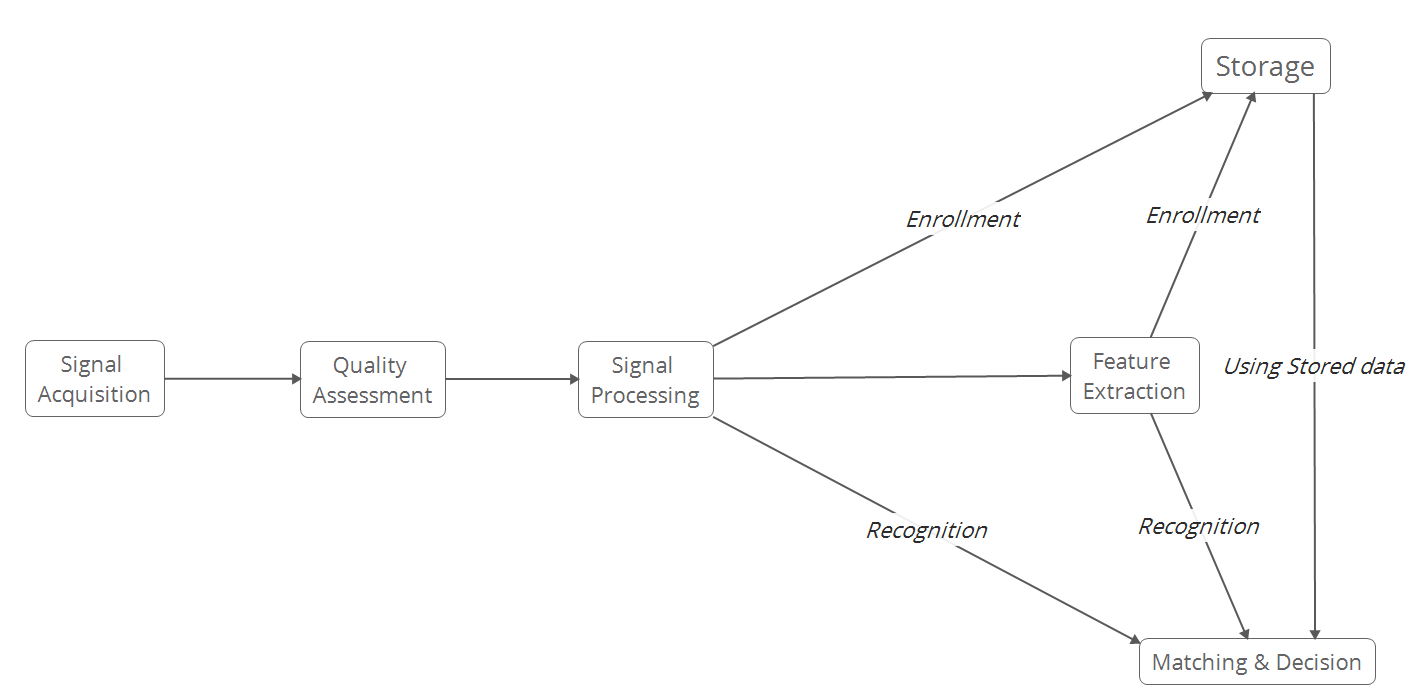
\includegraphics[width = .8\textwidth]{common_bio_process.png}
\caption{The common process for biometric system}
\label{fig:common_process}
\end{figure}

\subsection{Medical Biometrics}
Recently, medical biometrics, a new set of biometric signal are coming to forward(\parencite{Abo:2014biometric},\parencite{Agrafioti:2012secure},\parencite{Akhter:2016heart}, cited in \parencite{Pinto:2018evolution}). In general, medical biometrics depend on physiological characteristics, such as blood pressure, electrocardiogram (ECG), electroencephalogram (EEG), photoplethysmogram (PPG), etc.\parencite{Agrafioti:2011medical}. Table \ref{tab:comparision} shows the comparison among biometric traits.

\begin{table}

\centering
 \begin{tabular}{c c c} 
 Trait & Benefits & Drawbacks \\ [0.5ex] 
 \hline\hline
  & Universality & Requires contact \\ Electrocardiogram(ECG) & Hidden nature & Variability over time \\ & Simple acquisition & \\ 
 \hline
  & Universality & Expensive equipment \\ Electroencephalogram(EEG) & Hidden nature & Vulnerability to noise \\ &  & Variability over time \\ 
 \hline
  & Easily measurable & Easy circumvention \\ Face & Affordable equipment & Depends on face \\ & & Visibility and lighting \\ 
 \hline
  Fingerprint & High performance & Requires contact \\ & permanent over time & \\
 \hline
  Gait & Easy to measure & Low performance \\ & Affordable equipment & Variability over time \\
  \hline
  Iris & High performance & Expensive equipment \\
  \hline
  Palmprint & High measurability & Requires contact \\ & Permanent over time &  \\ 
  \hline
  & Easy to acquire & Low performance \\ Photoplethysmogram(PPG) & Hidden nature & Variability over time \\ & Affordable equipment & \\ 
  \hline
 Voice & Affordable equipment & Low performance \\ [1ex] 
 \hline
\end{tabular}
\caption{Comparison among biometric traits\autocite{Pinto:2018evolution}}
\label{tab:comparision}
\end{table}

Among those biometric traits, the ECG is the most promising signal for biometrics system\parencite{Pinto:2018evolution}. Because ECG is difficult to be falsified and can be used for liveness detection as it is a live indicator\parencite{Wang:2007analysis}. 

\subsection{Electrocardiogram}
The ECG signal describes the electrical activity of the heart over time. It is one of the most popular signals used for the health of human. To record ECG, a sensor should have at least two metal electrodes which must be contacted with the skin directly\parencite{Blasco:2018feasibility}.

\begin{figure}[H]
\centering
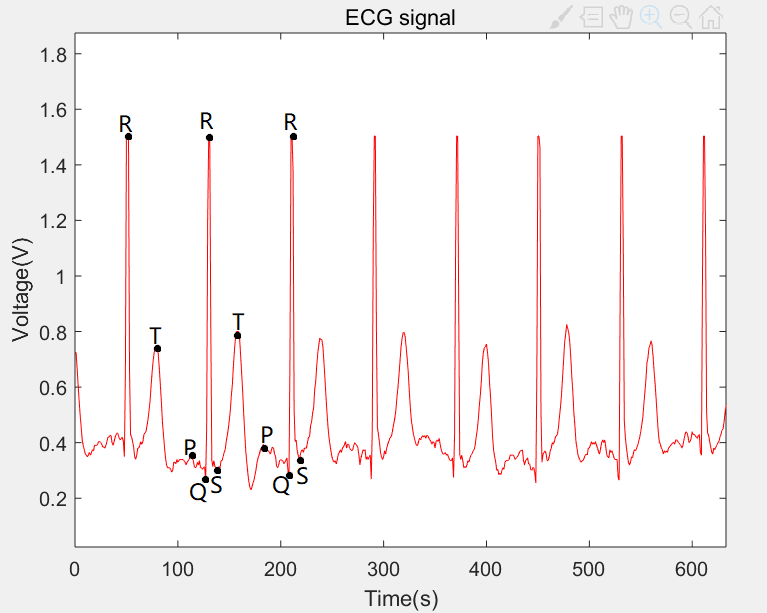
\includegraphics[width = .8\textwidth]{ecg.PNG}
\caption{ECG signals from BIDMC PPG and Respiration Dataset\autocite{PhysioNet}}
\label{fig:ecg}
\end{figure}

Biel et al.\autocite{Biel:2001ecg} is one of the earliest articles which introduce the possibility of using ECG for human identification. Fig \ref{fig:ecg} shows the main components which are used to identify humans include P wave, QRS complex and T wave. The P wave starts for the ECG signal, it represents the depolarization of the right and left atria\parencite{Agrafioti:2011heart}. The QRS wave is the largest wave, describes the depolarization of the ventricles\parencite{Wiki:ecg}. Finally, T wave is the end of a single ECG beat, which shows the repolarization of the ventricles\parencite{Lilly:2012pathophysiology}. For the ECG identification system, there are two main types: fiducial or non-fiducial\parencite{Agrafioti:2012secure}. In fiducial type, the peak of the R wave, T wave and P wave; the R-R interval, R-T interval are considered as features\parencite{Odinaka:2012analysis}. The non-fiducial based method does not use features, instead, some coefficients will be calculated as wavelet transform is used in Chan et al. \autocite{Chan2008wavelet}.

\subsection{Photoplethysmography}
Photoplethysmography (PPG) is a simple technique to detect blood volume changes at skin\parencite{Karimian:2017human}. PPG is widely used in fitness trackers and smart-watches to monitor user's fitness behavior and health statement. The sensors detect the light variations when blood passes through the skin\parencite{Blasco:2018feasibility}. PPG can be gathered from transmissive mode at the fingertip or reflection mode as on the forehead\parencite{wiki:ppg}. A common PPG is shown at Fig

\begin{figure}[H]
\centering
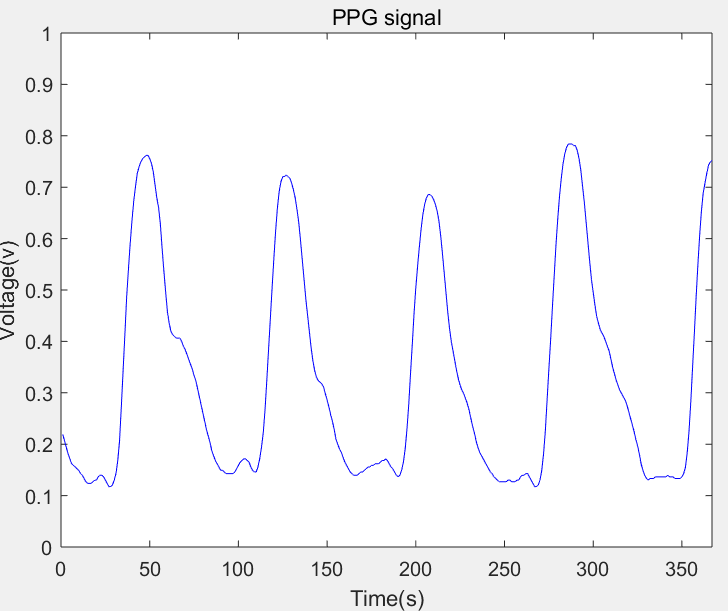
\includegraphics[width = .8\textwidth]{ppg.PNG}
\caption{PPG signals from BIDMC PPG and Respiration Dataset\autocite{PhysioNet}}
\label{fig:ppg}
\end{figure}

\subsection{Current Attacks}
As mentioned before, the biometric identification system does solve some problems in the traditional identification system, such as lost/forgotten because they are based on physical objects or the user's knowledge. However, nothing is perfect, biometrics leads into some brand-new risks. Fingerprint and face recognition are most common identification method, both can be easily observed and replicated by attacker\parencite{Eberz:2018your}. For example, fingerprints can be collected from a smooth surface like a glass cup. Moreover, face identification system might make a wrong decision because of a 2-D photo which is grabbed from victim's social media like Facebook.

Medical biometrics has become a popular research subject. In 2010, Odinaka et al. thought ECG are difficult to forge\parencite{Odinaka:2010ecg}. Agrafioti et al. mentioned the main strength of medical biometrics is robustness to reply, obfuscation and circumvention attack in 2011\parencite{Agrafioti:2011heart}.

However, even existing ECG biometrics are considered offering a high-security level against impersonation attacks\parencite{Blasco:2018feasibility}, it is not perfect, some attack has already been introduced. For instance, Eberz et al. present a presentation attack against ECG biometrics in Nymi band by reply previous ECG signals\parencite{Eberz:2017broken}. In the remainder of this section, we will discuss current attacks for both traditional biometrics and medical biometric.

\subsubsection{Attacks on traditional biometrics}
For traditional biometrics, the most common signals used to identify human is the face, fingerprint, and iris as static features, the voice is widely used to distinguish human as a dynamic signal when people make a phone call. However, because of the popularity of that method is so high that some high performance with low-cost attacks has already existed.

In 2012, Galbally J et al. \autocite{Galbally:2012iriscode} introduced an attack based on iris code to rebuild origin iris information. The experimental result showed that the reconstructed images are very realistic and might have a chance to break through the iris identification system. As their result, the possibility for unauthorized access is 75\% to 94\%.

In 2015, Ergünay S K et al. \autocite{Ergunay:2015voicevulnerability} introduced a voice spoofing data-set which include threat contain reply, speech synthesis, and voice conversion. Also, an experimental were provided to show the effect to an automatic speaker verification system. The spoofing false acceptance rate is 96.5\% for Male and 81.5\% on Female.

In 2017, Chen et al. \autocite{Chen:2017spoofing}researched a method to spoofing faces by using makeup. They found automated face recognition machine are suffered from makeup attack. They thought it is easy for the malicious individual to trick identification system by using makeup. However, the worst case for identification in their research is around 50\% when testing 30 probe image with commercial Off-The-Shelf face software.

\subsubsection{Attacks on medical biometrics}
Traditional biometric features are suffered from forge attack but the medical biometric features like ECG are not easy to counterfeit because of the uniqueness of the signal for the individual. However, since 2003 the dynamical method for generating ECG was provided by McSharry P E et al. \autocite{Mcsharry:2003dynamical} the forge attack to ECG became possible. In their research, the operator can specify the mean and deviation of the heart rate, the power of R and shape of the PQRST cycle. The attacker might generate a realistic ECG signal to access the ECG identification system.

Moreover, In 2017, Eberz et al. \autocite{Eberz:2017broken} provided an attack target on ECG biometric identification system. They demonstrate the attack based on the Nymi band which is a wrist band as a biometric identification system. The attack based on reply the ECG signal which captured previously. The result of the attack, 81\% success rate for the best case which used the signal collected from Nymi band, for remaining signal sources like the signal collected from medical ECG monitor, the success rate is 62\%. In the same year, Karimian N, Woodard D L, and Forte D introduced another presentation attack\parencite{Karimian:2017vulnerability} which map the attacker's ECG to victim's by using captured victim's ECG. The mapping function is suitable for both off-line attack and online attack which attacker has less time and resources. For the experiment result, the average success rate is 97.43\% and 94.17\% towards non-fiducial and fiducial based ECG identification system respectively. In the online mode, the performance decreased for 5.65\% in the non-fiducial system but unaffected on the fiducial system.

\subsection{Motivation}
Although those attacks on ECG are novel, the effect is limited because they assume the ECG signal of a victim has already captured\parencite{Blasco:2018feasibility} and reply attack on ECG can be easily detected by computing the hash, because due to the sample rate and the particularity of the ECG signal, each hash must be different. Simultaneously, PPG is widely used in wearable devices and much easier collect than ECG, especially when a remote PPG collection method is introduced by Verkruysse et al. which can collect PPG remotely (> 1m) with ambient light by inexpensive digital cameras (< \$200)\parencite{Verkruysse2008remotePPG}. In addition, because of both ECG and PPG are represented the motivation of heart and the synchronized ECG and PPG signals are shown in Fig \ref{fig:ppg_ecg}, we thought there might be some correlations between PPG and ECG. Thus, we decided to find a transfer formula by using the neural network to generate ECG against ECG identification system from the collected PPG.

\begin{figure}[H]
\centering
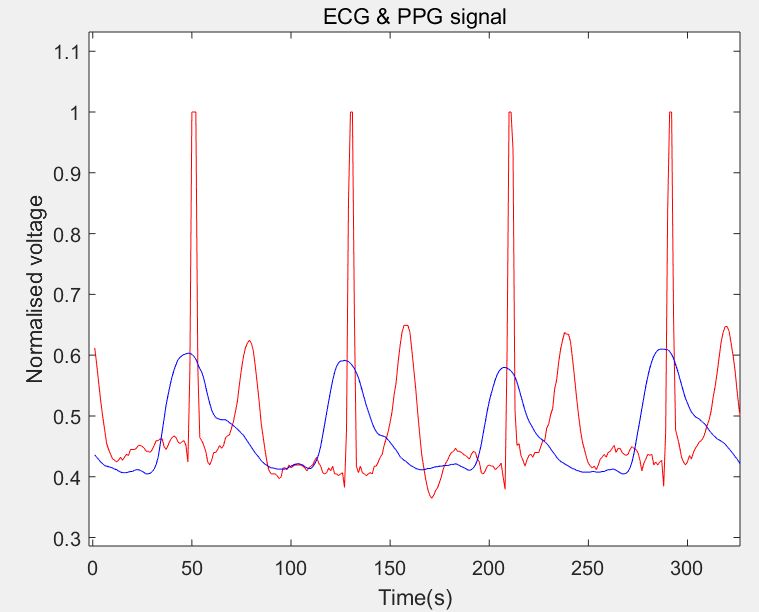
\includegraphics[width = .8\textwidth]{ecg_ppg.PNG}
\caption{Synchronized ECG and PPG signals from BIDMC PPG and Respiration Dataset\autocite{PhysioNet}}

\label{fig:ppg_ecg}
\end{figure}

\section{Machine Learning}
\subsection{Machine Learning in Authentication}
\subsection{Neural Network}

\section{Related Work}

\section{Conclusion}

\printbibliography

\end{document}
